\documentclass{article}
\usepackage[letterpaper]{geometry}
\usepackage{graphicx}
\usepackage{hyperref}
\usepackage{amssymb, amsmath, charter, latexsym}
\usepackage{ragged2e}
\usepackage{mathptmx}
\usepackage{listings}
\usepackage{siunitx}
\usepackage{booktabs}
\DeclareMathOperator*{\argmin}{arg\,min}
\DeclareMathOperator*{\argmax}{arg\,max}
\newcolumntype{P}[1]{>{\centering\arraybackslash}p{#1}}

\lstset{
basicstyle=\ttfamily,
}
\lstMakeShortInline|

\begin{document}

\title{\bfseries ECEN 689 -- Real-Time Wireless Networks: Project 3\\
S-WiFi: Smart Scheduling with Point Coordination Function for WiFi Uplink Transmissions}
\date{Due on 5/6}
\author{%
Ping-Chun Hsieh\\
\texttt{lleyfede@tamu.edu}
\and
Tao Zhao\\
\texttt{alick@tamu.edu}
\and
Dongni Han\\
\texttt{handongni2015@tamu.edu}
}
\maketitle

\section*{Terminology}

In our report, we use AP or ``server'' to denote the WiFi access point, and ``client'' to denote the terminal device such as a mobile phone, a tablet, and so on. Throughout our simulation, we let node $0$ be the server, and the other nodes be the clients. The basic time unit for packet transmission is called \emph{slot}, which should be greater than a round-trip time (RTT). For real-time traffic, we group an integer number (denoted by $T$) of slots into an \emph{interval}, which is the relative deadline of the packets.

\section{Background}
\subsection{System Model}
We consider a wireless network of one AP and $N$ clients, where $N\ge1$. We consider uplink transmissions with point coordination function (PCF) for real-time traffic. We assume packets are generated by each client $n$ in the beginning of each interval. The number of packets generated by client $n$, denoted by $X_n$, follows a uniform distribution in the range of [$U_{\min}$, $U_{\max}$]. In PCF mode, the AP has centralized control of client scheduling, and polls at most one client per slot. The clients wait for the AP's message to access the wireless channel. In this way, collisions are avoided. Whether a scheduled transmission is successul or not depends only on the channel reliabilities denoted by $p_n$. Figure~\ref{fig:network} illustrates the system model with three clients.

\begin{figure}[htbp]
   \centering
   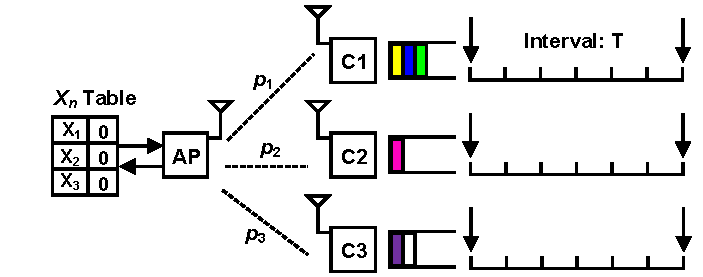
\includegraphics[width=\textwidth]{../presentation/network.pdf}
   \caption{An example of the system: $N=3$}
   \label{fig:network}
\end{figure}

The main challenge of using PCF for WiFi uplink transmissions is that since the packets are generated and queued on the client's side, and the AP does not know the number of packets of each client at first. Therefore, the AP needs to collect the queue information of the clients to make scheduling decisions.

\subsection{Baseline Policy}
Under the baseline policy, the AP first collects the queue information by polling each client one by one for the number of data packets it generates ($X_n$). After all clients are polled, the AP knows the number of packets at each client. Next, the AP uses the Max-Weight policy to schedule one of the clients in each time slot for actual data transmission, where the weight is the product of the remaining queue length and the channel reliability for each client.

The major issue of the baseline policy is that there is no data transmission in the first phase of polling queue information $X_n$. As a result, channel utilization for data packets can be very low. In fact, we have shown in the previous project that the channel utilization is especially low with large network size (large $N$) or poor wireless channels (small $p$) since the AP ends up spending most of the time on polling queue information $X_n$.

\section{Smart Policy}

To address the issue of the baseline policy, we propose three different features to improve the network performance, and integrate them together in our smart policy.

\subsection{Selective Polling}
The first feature is selective polling. In each interval, the AP only polls the queue information of a subset of $n \le N $ clients. By properly choosing $n$, the AP avoids spending too much time on polling queue information while collecting enough queue information for scheduling. The algorithm of determining the optimal $n$ includes the following three steps:
\begin{enumerate}
\item Sort the clients by their channel reliabilities so that $p_1 \geq p_2 \geq \dots \geq p_N$;
\item Calculate the estimated total timely-throughput of $n$ clients by
   \[
   \hat{R}_n = \min\left\{n\frac{U_{\min}+U_{\max}}{2}, \left(T-\sum_{i=1}^{n}\frac{1}{p_i}\right)\frac{\sum_{i=1}^{n}p_i}{n} \right\};
   \]
\item Find the optimum $n^* = \argmax_{n} \hat{R}_n$.
\end{enumerate}
Step 1 is based on the intuition that clients with better channel reliabilities can deliver better throughput. The sorting allows us to look at only the first $n$ clients with good channels, instead of looking at all the subsets of clients with cardinality $n$. In step 2, we compare the total number of packets generated on average, $n\frac{U_{\min}+U_{\max}}{2}$, with the number of packets that can be potentially delivered in the remaining slots for data transmissions in one interval. Here $\left(T-\sum_{i=1}^{n}\frac{1}{p_i}\right)$ serves as an estimate of the average number of slots available for data packets, and $\left(\frac{\sum_{i=1}^{n}p_i}{n}\right)$ is the average channel reliability of this subset of clients.

After we get the number of seleted clients $n$, we need to determine the subset with $n$ clients. Although the above algorithm suggests the $n$ clients with largest channel reliabilities, we choose to draw a random permutation for better fairness among the $N$ clients in the implementation.
Random permutation can be realized by the famous Knuth shuffle algorithm.

Note that it might be possible that all the selected clients are served completely ahead of the end of the interval. In such case, considering the number of the remaing time slots are limited, we will serve the remaining clients one by one.

\subsection{Piggybacked Queue Length}

Another idea to migiate the polling overhead is to allow piggybacked queue information. When a client receives a polling message, it replies with its queue length $X_n$ as well as the first data message (if there is any) in one packet to the AP. Hence, all slots become effectively available for data transmission. Consequently, when this feature is combined with selective polling, the estimated throughput used in selective polling should be modified as
\[
\hat{R}_n = \min \left\{n\frac{U_{\min}+U_{\max}}{2}, T \frac{\sum_{i=1}^{n}p_i}{n} \right\}.
\]

To implement this feature in ns-2, we introduce two new packet types: \lstinline|SWiFi_PKT_POLL_PGBK| for the AP to poll clients and \lstinline|SWiFi_PKT_PGBK_UL| for the clients to reply their piggybacked information. The queue information is maintained in the header of \lstinline|SWiFi_PKT_PGBK_UL| packets.

\subsection{Retry Limit for Polling}

The last idea we come up with is to impose retry limit for polling queue information.
Consider a network where one of the clients has almost zero channel reliability. Under the baseline policy, the AP will with high probability keep polling the queue information of that client indefinitely in each interval and end up producing zero timely-throughput. As a countermeasure, retry limit for polling can prevent the AP from spending too much time on polling clients with poor channels, and thus achieve better timely-throughput.

To implement this feature, we choose to disable the built-in retry function of 802.11 MAC and handle retransmission completely in the application layer. This allows us to have full control over the timing of retransmissions. We introduce a variable \lstinline|num_retry_| to keep track of the number of retries. When the AP starts polling a new client, \lstinline|num_retry_| is set to 0. \lstinline|num_retry_| increases by 1 after each polling retry. If the retry limit is reached, the AP then starts polling the next client regardless of the result of the last transmission.

\subsection{Integrated Policy}
Our smart policy combines selective polling, piggybacked queue length, and retry limit for polling together as an integrated policy. In each interval, the AP first determines the selected clients by selected polling. Then it sends out the \lstinline|SWiFi_PKT_POLL_PGBK| packet to each selected client, and expects piggybacked replies. The maximum number of retries for polling the queue information of each client is given by the retry limit. If there are still time slots in the interval after all selected clients are served, the remaining clients will be served one by one.

For better modularity, our implementation in fact allows us to enable or disable the above three features independently. We use binary digits to represent different features. Hence, the policieshave their corresponding binary numbers. All possible policies and their binary representation are listed in Table~\ref{Policy Types}. As a special case, the baseline policy is essentially one with all three features disabled (000).

\begin{table}[htbp]
   \centering
   \caption{Policy types and binary representation.}
   \label{Policy Types}
   \begin{tabular}{| P{4cm} | P{3.5cm} |}
       \hline
       Policy Types   &  Binary representation\\   \hline
       Baseline &  000\\ \hline
       Selective & 001\\ \hline
       Piggyback & 010\\ \hline
       Selective + Piggyback & 011\\ \hline
       Retry Limit  &100\\ \hline
       Selective+ Retry Limit & 101\\ \hline
       Piggyback + Retry Limit & 110\\ \hline
       Smart &  111\\
       \hline
   \end{tabular}
\label{table: policy}
\end{table} 

\section{Simulation Results}
\subsection{Simulation Setup}
\label{section: simulation: setup}
Throughout the simulation, we consider a network of one AP and 5 clients unless stated otherwise. We use the shadowing module as the wireless channel. The parameters of the channel are shown in Table \ref{table: channel}. The transmitter power is $\SI{1}{W}$, and the channel reliability is varied by changing the distance between the AP and the clients. 

\begin{table}[htbp]
\centering
    \caption{Parameters of the wireless channel.}
    \vspace{2mm}
    \begin{tabular}{ | l | l | }
    \hline
    Item & Value \\ \hline
    Path loss exponent & 2.0  \\ \hline
    Shadowing deviation & \SI{4.0}{dB} \\ \hline
    Reference distance & \SI{1.0}{m} \\
    \hline
\end{tabular}
\label{table: channel}
\end{table}

\begin{table}[htbp]
\centering
\caption{Parameters of the 802.11b MAC.}
    \vspace{2mm}
    \begin{tabular}{ | l | l | }
    \hline
    Item & Value \\ \hline
    Data rate & \SI{11}{Mb/s}  \\ \hline
    Basic rate & \SI{1}{Mb/s}  \\ \hline
    PLCP data rate & \SI{1}{Mb/s}  \\ \hline 
    Preamble length & \SI{144}{bits} \\ \hline
    Slot time & \SI{20}{\mu s} \\ \hline
    SIFS & \SI{10}{\mu s} \\
    \hline
\end{tabular}
\label{table: mac}
\end{table}

For the medium access control (MAC) layer, we use the 802.11 MAC module built in ns-2 and the key parameters are summarized in Table \ref{table: mac}. As mentioned earlier, we disable the automatic retransmission function of 802.11 MAC by letting \lstinline|ShortRetryLimit_| and \lstinline|LongRetryLimit_| be 1 in the Tcl script \lstinline{swifi.tcl}.

In the application layer, 1 time slot is chosen to be $\SI{10}{ms}$ to leave enough margin for data transmission. The key simulation parameters are summarized in Table \ref{table: parameter}. In the fully-symmetric case, we let $p_i = p$, for any client $i$. In the asymmetric scenario, we let $p_1 = p_2 = 1$ and $p_j = p$, for $j = 3, ..., N$. We use the timely-throughput of the network as our primary performance metric to evaluate different scheduling policies. We report the average throughput values over 10 simulation runs.

\begin{table}[htbp]
\centering
    \caption{Simulation parameters.}
    \vspace{2mm}
    \begin{tabular}{ | l | l | }
    \hline
    Item & Value \\ \hline
    Slot time & \SI{10}{ms}  \\ \hline
    Interval length & \SI{10}{slots} \\ \hline
    $U_{\min}$ & 0 \\ \hline
    $U_{\max}$ & 2 \\ \hline
    Retry limit & 1 \\ \hline
    Simulation runs & 10 \\
    \hline
\end{tabular}
\label{table: parameter}
\end{table}

%Each interval contains 10 time slots. The number of packets generated follows uniform distribution in the range of $U_\text{min}=0, U_\text{max}=2$. Channel reliability $p\approx0.57$ which its distance is \SI{1000}{m}. Retry limit is one. Every 

\subsection{Performance Over Symmetric Channels}
We first evaluate the policies in the fully-symmetric scenario. Figure \ref{sim: sym: smart and baseline} shows the network timely-throughput with different channel reliabilities under the smart policy and the baseline policy. The smart policy achieves larger timely-throughput than the baseline policy regardless of the channel reliability. In particular, the smart policy makes the most significant difference when the channel reliability is moderate. Moreover, the smart policy is able to deliver all packets when $p=1$ while the baseline policy can not. This is because the baseline policy spends half of the interval on polling queue information so that there are only 5 slots left for data transmission.

\begin{figure}[htbp]
\centering
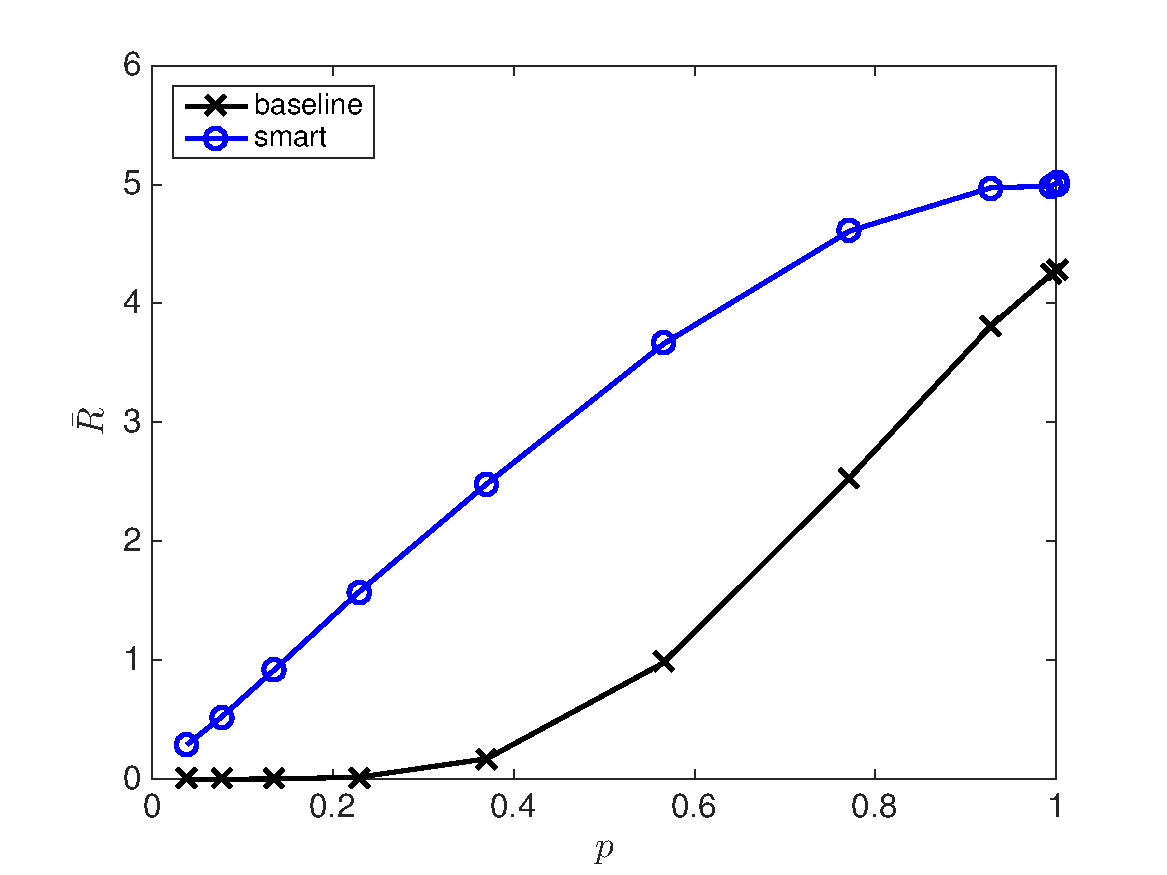
\includegraphics[scale=0.5]{R_p_sym.pdf}
\caption{Throughout versus channel reliability in the fully-symmetric scenario.}
\label{sim: sym: smart and baseline}
\end{figure}

Next, we evaluate the performance of each individual feature. Figure \ref{sim: sym: three features} shows the timely-throughput with the selective, piggyback, and the retry limit feature in the fully-symmetric case. Among the three features, the piggyback function provides the most performance gain regardless of the channel condition. The selective or the retry limit function also individually improves the network timely-throughput when the channel reliability is less than 0.8. This is because the polling overhead under the baseline policy becomes much more significant when the channel is less reliable. Figure \ref{sim: sym: combined} further shows the performance of the policies with two combined features. In the symmetric scenario, the piggyback feature per se already achieves similar performance as the smart policy.

\begin{figure}[htbp]
\centering
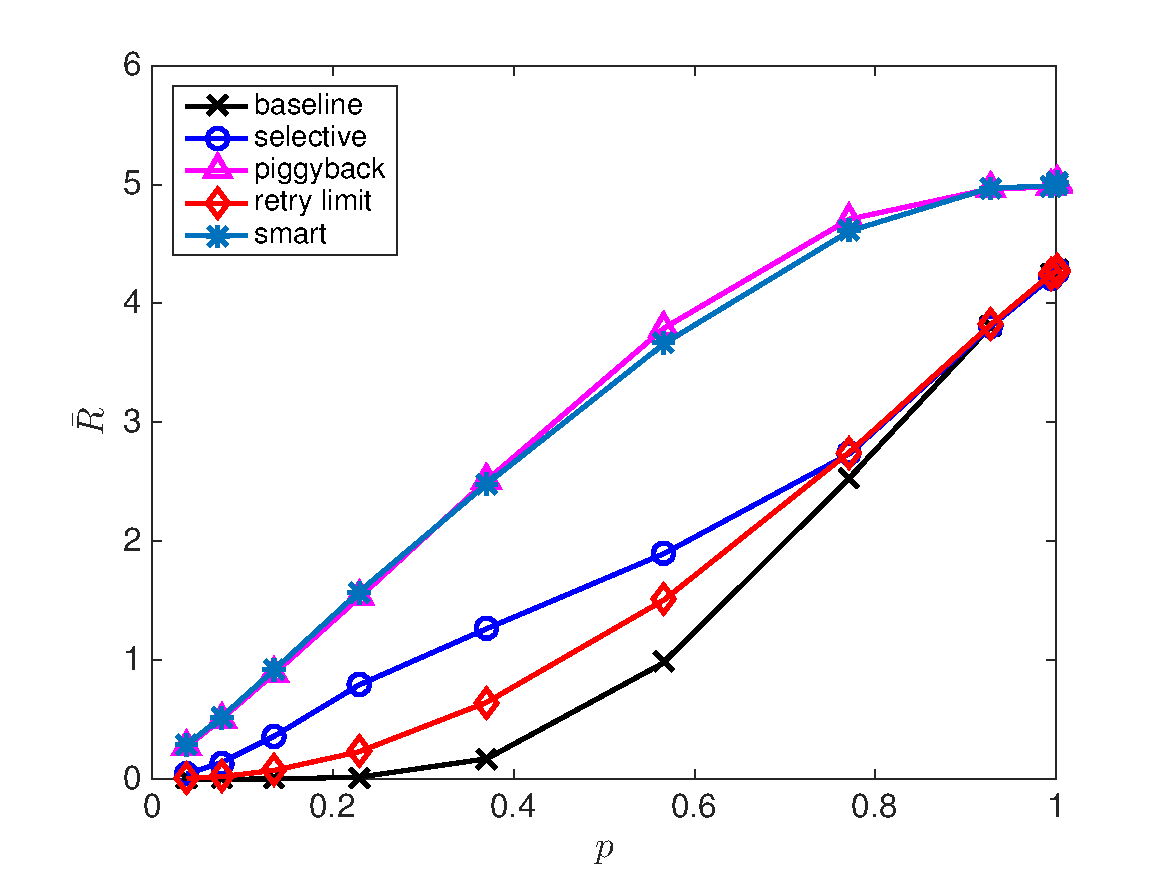
\includegraphics[scale=0.5]{3policycompare_sym.pdf}
\caption{Throughout versus channel reliability in the fully-symmetric scenario: baseline, smart, and polices with each individual feature.}
\label{sim: sym: three features}
\end{figure}
\begin{figure}[htbp]
\centering
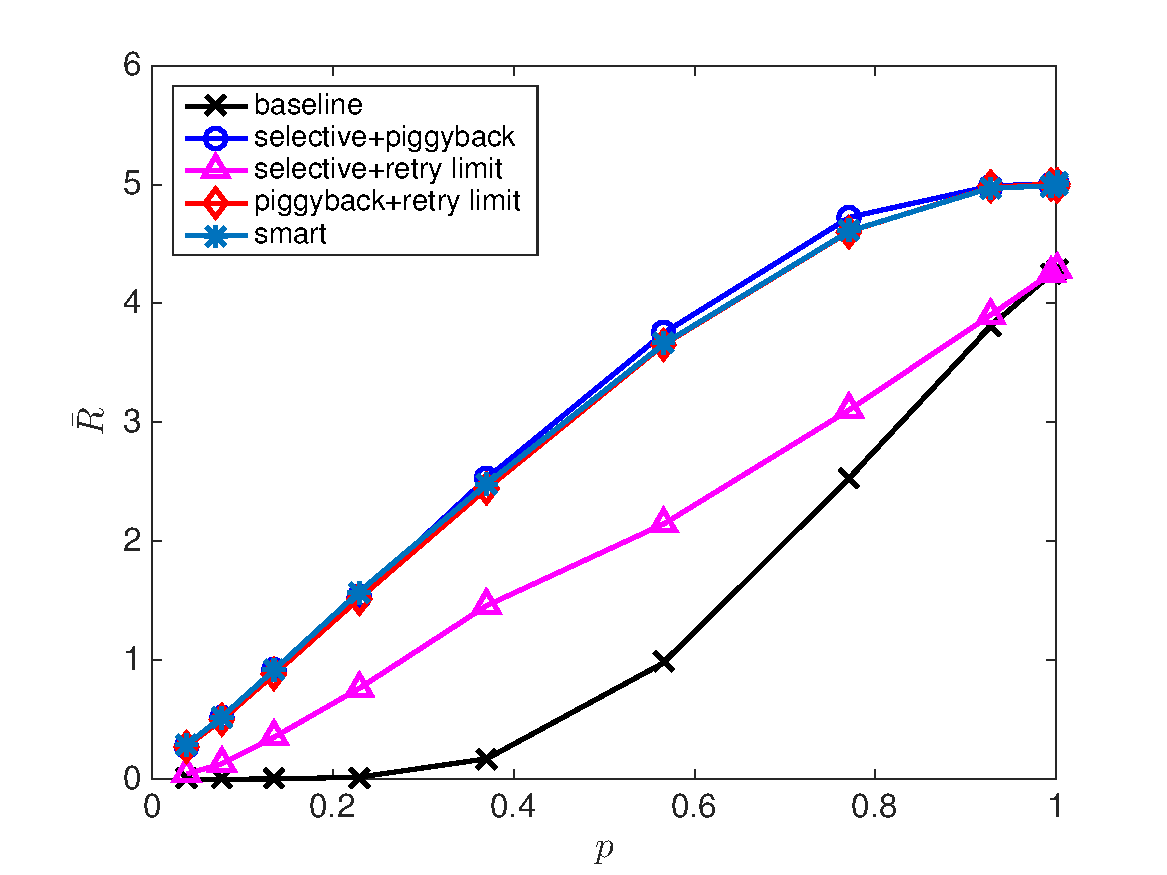
\includegraphics[scale=0.5]{sym_threecombinepolicys.pdf}
\caption{Throughout versus channel reliability in the fully-symmetric scenario: baseline, smart, and polices of two features.}
\label{sim: sym: combined}
\end{figure}

We are also interested in the effect of network size on the overall performance. Figure \ref{sim: sym: different N} shows the total timely-throughput with different number of clients and the channel reliability $p \approx 0.57$. The smart policy performs steadily when the number of clients increases from 5 to 10. On the other hand, the baseline policy provides nearly zero timely-throughput when there are more than 8 clients. This shows that the smart policy also achieves much better scalability. Note that when there are only two clients, our smart policy performs slightly worse than the baseline policy. This is because in such a small size network, retry limit of one is too conservative. With a larger retry limit, our smart policy can again performs better than the baseline policy.

\begin{figure}[htbp]
\centering
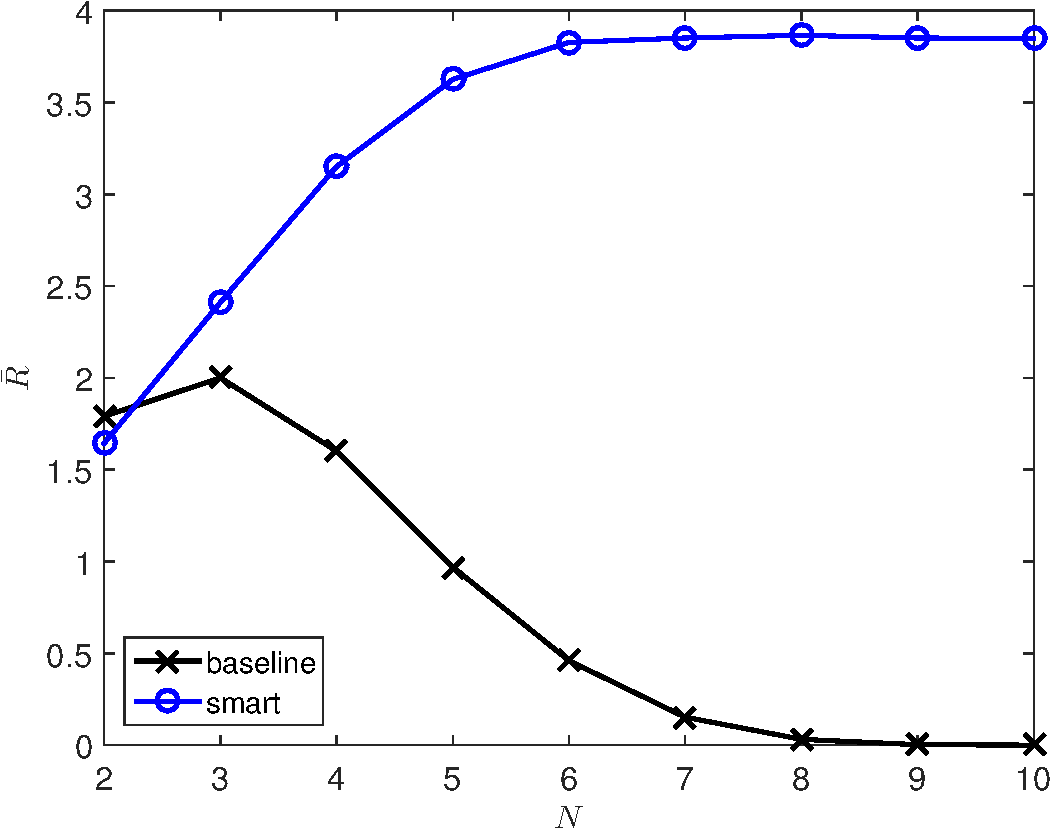
\includegraphics[scale=0.5]{R_N_sym.pdf}
\caption{Throughout versus number of clients in the fully-symmetric scenario.}
\label{sim: sym: different N}
\end{figure}

%Figure \ref{smart and baseline asym} shows smart policy and Baseline policy under asymmetric channel. smart policy is consistently better under asymmetric channel, especially when the channel is poor. \\

%Figure \ref{Combined Policies Under Symmetric Channel} shows Baseline, Selective + Piggyback, Selective + Retry Limit, Piggyback + Retry Limit and smart policy under symmetric channel. Selective + Piggyback is the best and it is even better than smart policy. smart and Piggyback + Retry Limit are equal, which implies that Piggyback and Retry Limit play vital roles among these three features. The worst combined policy is Piggyback and Retry Limit. \\

\subsection{Performance Over Asymmetric Channels}
We also evaluate the performance over asymmetric channels.
Figure \ref{sim: asym: three features} shows the performance of the baseline policy, the smart policy, and the policy of each individual feature over different channel reliabilities for the distant clients. Again, we can find our smart policy provides significant improvement over the baseline policies regardless of the channel conditions.
Among the three features, the piggyback function still achieves the most improvement. Different from the symmetric case, the piggyback feature by itself can not achieve the same performance as the smart policy when $p$ is fairly small. This is because that the piggyback feature is not able to prevent the AP from spending too much resource on the clients with very poor channel. Besides, the retry limit feature provide more performance gain than the selective polling feature when the channel is not quite good. Interestingly, the retry limit feature exhibits convexity in total timely-throughput when $p$ is between 0 to 0.4. This is because when $p$ is extremely small, the AP can not receive the queue information from these distant clients. Therefore, the AP gives up data transmissions for them, and serve the client with better channels instead.

\begin{figure}[htbp]
\centering
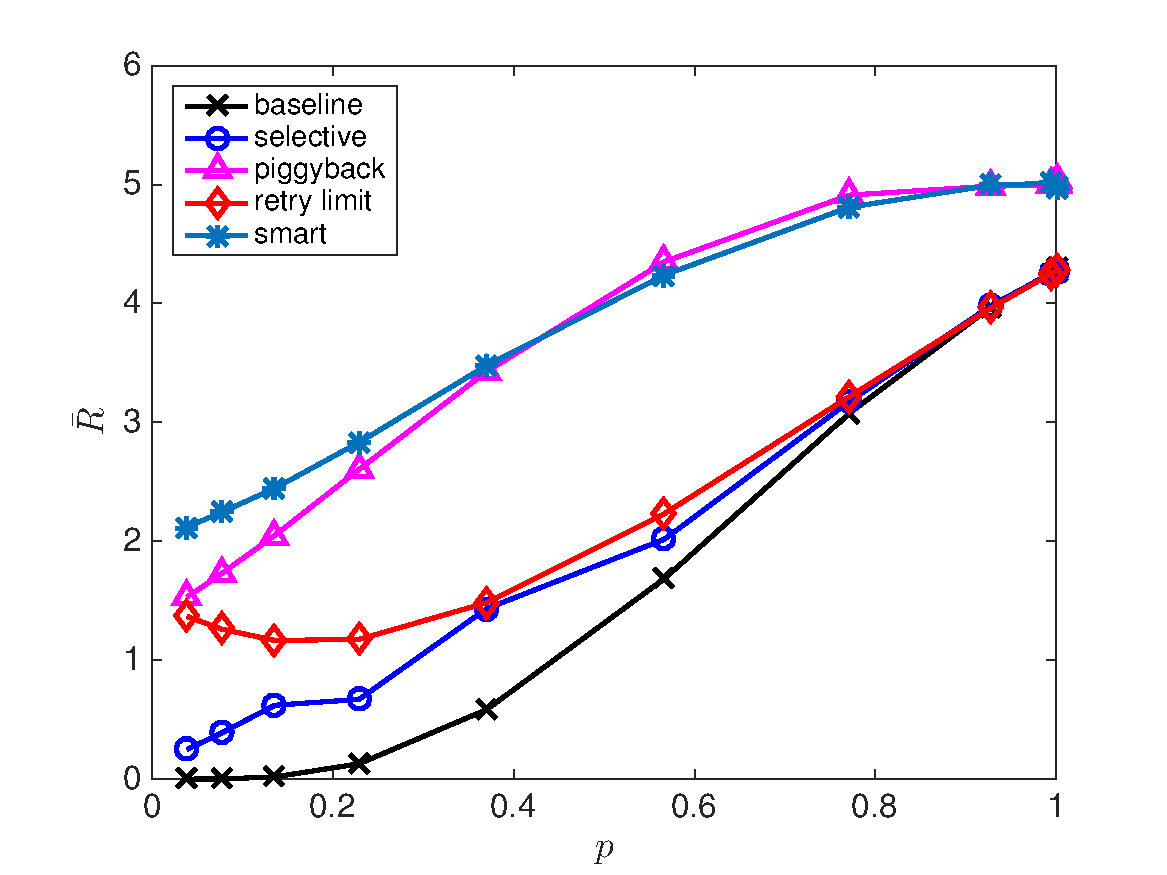
\includegraphics[scale=0.5]{3policycompare_asym.pdf}
\caption{Throughout versus channel reliability in the asymmetric scenario: baseline, smart, and policies with each individual feature.}
\label{sim: asym: three features}
\end{figure}

Next, we evaluate the policies with two combined features, as shown in Figure \ref{sim: asym: combined}. In our asymmetric scenario, the policy with piggybacked queue length plus retry limit can achieve similar performance as the smart policy. Therefore, it is worth studying the possible scenarios where the selective polling feature provides further timely-throughput gain in the smart policy.

\begin{figure}[htbp]
\centering
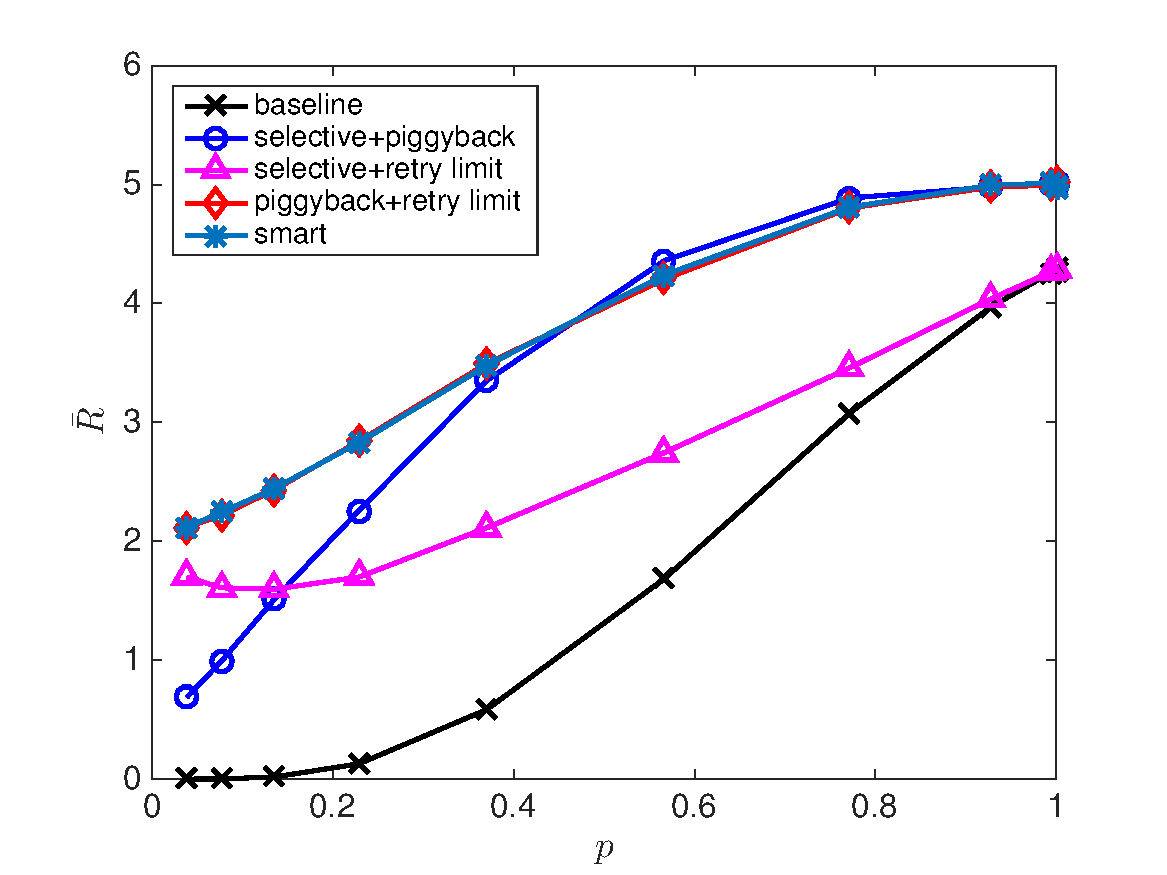
\includegraphics[scale=0.5]{asym_threecombinepolicys.pdf}
\caption{Throughout versus channel reliability in the asymmetric scenario: baseline, smart, and polices of two combined features.}
\label{sim: asym: combined}
\end{figure}

%Figure \ref{Combined Policies Under Asymmetric Channel} shows Baseline, Selective + Piggyback, Selective + Retry Limit, Piggyback + Retry Limit and smart policy under asymmetric channel. When channel reliability $p$ is smaller than 0.15, Piggyback and Retry Limit are the same. Then Selective + Retry Limit is better than Selective + Piggyback. However, Selective + Piggyback becomes better than Selective + Retry Limit when channel reliability $p$ is larger than 0.15. When channel reliability $p$ is larger than 0.5, Selective + Piggyback is the best. When channel reliability $p=1$, the system delivers all packets under Selective + Piggyback, smart and Piggyback + Retry Limit. \\

Finally, we also evaluates the performance of the policies in terms of network utility. We define the utility of each client $n$ as
\[
U_n(q_n)=\log \left(\frac{q_n}{10^{-4}}\right) ,
\]
where $q_n$ is the timely-throughput for client $n$.\footnote{The constant $10^{-4}$ is only an offset to get more readable utility values.}
The network utility is the summation of the utility for all clients:
\[
U = \sum_n U_n(q_n) = \sum_n \log (\frac{q_n}{10^{-4}}) .
\]
This utility function corresponds to proportional fairness in network utility maximization problems. Figure \ref{sim: asym: utility} shows the network utility with different channel reliabilities in the asymmetric scenario. It is clear that the smart policy achieves much better utility than the baseline policy under different channel conditions. This indicates that our smart policy also maintains a higher level of fairness across the network.

\begin{figure}[htbp]
\centering
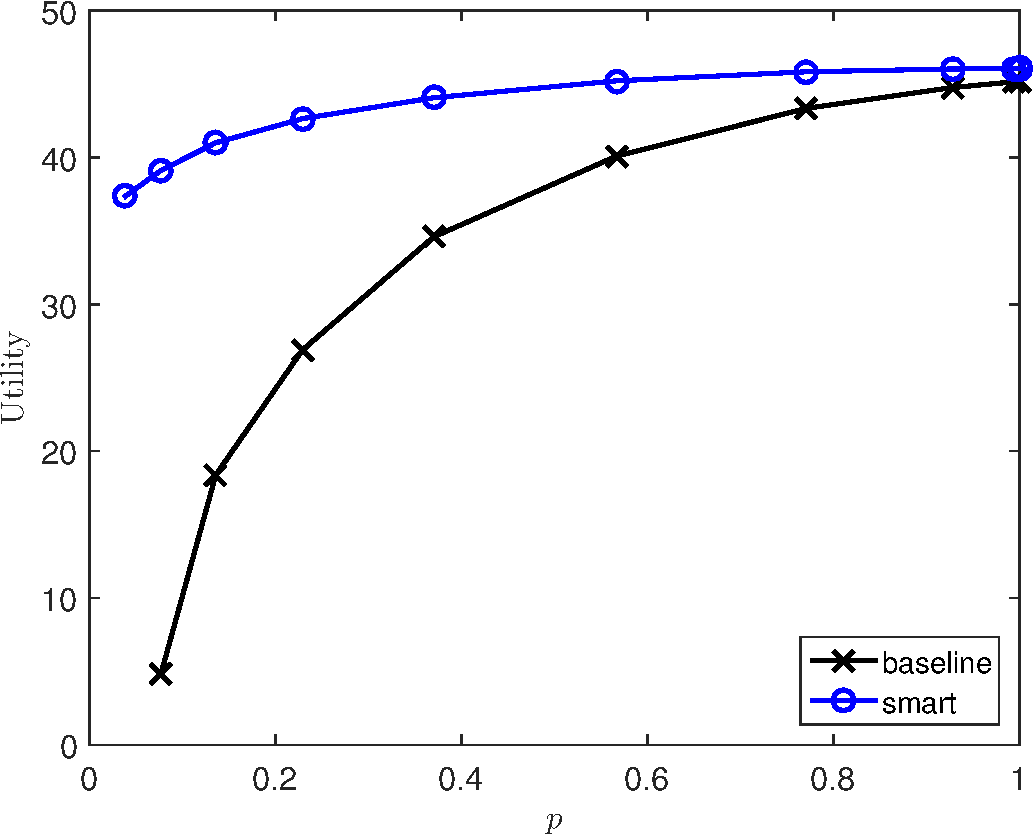
\includegraphics[scale=0.5]{U_p_asym.pdf}
\caption{Network utility versus channel reliability in the asymmetric scenario with $p\approx 0.57$.}
\label{sim: asym: utility}
\end{figure}

\section{Conclusion}

We present the design and implementation of S-WiFi, which utilizes a smart scheduling policy for WiFi uplink transmissions in PCF mode. Our smart policy incorporates selective polling, piggybacking, and retry limit to improve the system performance. Simulation study shows the smart policy outperforms the baseline policy in terms of timely-throughput and network utility in various network settings.

\appendix
\section{Source Code}
The source code of S-WiFi can be found on \href{https://github.com/S-WiFi/S-WiFi}{GitHub}.
\end{document}
